\providecommand{\MainFolder}{..}
\documentclass[\MainFolder/Text.tex]{subfiles}
\begin{document}
\addchap*{Acknowledgements}
\Modify[noline]{DONE Check who has Dr. in name!}

First and foremost, I thank my parents, \emph{Dana H\'ajkov\'a} and \emph{Libor H\'ajek,} for supporting me throughout my studies, both emotionally and materially, for discussing various decisions I had to make, for listening when I needed to talk and for wishing me all the best in whatever I wanted to~do.
%and never left me alone or condemned me even in times when I was not the nicest to them.
D\'iky moc mami a tati!

I thank my grandparents,  And\v{e}la H\'ajkov\'a, Anna Uhl\'ikov\'a and Jaroslav Uhl\'ik, for their love and support, although they would rather see me being happy and having a family than pursuing a doctorate. D\'iky moc babi a d\v{e}do! \Add[noline,caption={DONE Add cross}]{DO NOT Add cross to Anna Uhlikova}

Next, I thank my supervisor, Prof.~Dr.~Kai Cieliebak, for giving me time and support to get through the graduate studies, to develop academically and to finish the thesis. I~enjoyed discussions with him very much and learned from his insights and methods. I~appreciate and admire his skill to explain everything anytime starting from elementary facts, his passion for mathematics and physics, scientific productivity and lecturing skills. Danke sch\"on, Kai!
%I also thank my grandparents Jaroslav Uhlik, Anna Uhlikova and Andela Hajkova for their support.
%Then general and funny thanks.
%``A. Grothendieck: Fertility is measured by offspring, not by honours.''
%I am still not sure whether the globalized world connected by the internet media. The internet is It is indeed terrible.

%I thank Prof.~Dr.~Janko Latschev for giving me a postdoc position in Hamburg and for letting me finish the thesis even after a couple of deadlines which we agreed on (except for the last one). Vielen Dank, Janko!

%, for offering me a position in Prague and for discussions. D\'iky Bra\v{n}o, p\v{r}\'i\v{s}\v{t}e v Praze!

I thank Dr.~Evgeny Volkov for discussing his work on Chern-Simons theory, string topology, cyclic homology and Chen's iterated integrals, for providing me his preprints in progress and for supportive chats at the university. Thank you, Evgeny, good luck fighting with lions in Siberia!

I~thank Prof.~Robert Bryant for proposing an alternative notation for the Hodge propagator for spheres in an online discussion. I thank Prof.~John Rognes for answering my question about spectral sequences in an online discussion. I thank Dr.~Najib Idrissi for answering my question about formality in an online discussion. I also thank the online discussion --- Mathoverflow and Math Stackexchange --- for its existence.

I~thank Dr.~Alexandru Doicu for checking a tedious sign computation and for friendly talks. I~thank Dr.~Andreas Hermann for discussing the standard Hodge propagator, for sending me his notes on the Green kernel for spheres and for his interest in my work. I~thank Prof.~Dr.~Hông Vân Lê for discussing her work on formality and Poincar\'e $\DGA$'s and for her interest in my work. I thank J\'an Pulmann and Lada Peksov\'a for discussing $\BV$-formalism and properads. I thank Ond\v{r}ej~Hul\'ik for a Skype discussion about physics and for friendly talks. I thank Ji\v{r}\'i Zeman for pointing out that absolute convergence is equivalent to invariance on resummations and for friendly talks. I thank Dr.~Kyler Siegel for a discussion about A-infinity in Stony Brook. I thank Dr.~Raymond Puzio for his interest in my work, for thinking about an action for our propagator and for friendly talks. I~thank Prof.~Alberto Cattaneo and Dr.~Pavel Mnev for discussing Feynman integrals and an action for our propagator in Stony Brook and for sending me a list of relevant literature later. I~thank Prof.~Dr.~Bra\v{n}o Jur\v{c}o for discussing $\BV$-formalism and for offering me a position in Prague.

I thank Prof.~Dr.~Christian~B\"ar, Prof.~Dr.~Kaoru Ono and Prof.~Dr.~Janko Latschev for inviting me to their institutes to discuss and give a talk, for their hospitality and for valuable feedback and insights. I am grateful to Prof.~Dr.~Janko Latschev for giving me a position in Hamburg and for waiting until I finish the thesis.

Although everything mentioned in the last paragraphs occurred in the final fifth year of my Ph.D., it inspired me and motivated me to complete the work.

I thank members of the department for mathematics at the University of Augsburg for creating and maintaining a rich and inspiring academic environment. I thank Prof.~Dr.~Urs Frauenfelder for various discussions and for always coming up with a highly interesting topic for the symplectic seminar, which, at the beginning, I often preferred to my own work. I~thank Prof.~Dr.~Edward Belbruno, a~visiting professor from Princeton, for his series of talks about chaotic dynamics in celestial mechanics, for the explanation of the weak stability boundary, for organizing exciting events related to space travel and for stopping by our office to chat about various topics.

I thank my colleagues at the university; those who I liked for being friendly and encouraging, and those who I did not for putting up with me and for not fueling conflicts. Specifically, I thank Alexei Kudryashov and Thorsten Hertl, who hanged out with me in the final two years when I was spending the most of my time at the university, and who had to listen to my laments about lost years, starting to work on concrete problems too late, terrible topic which is not geometric at all, internet overuse and screwed up personal life. I can not forget to highlight their top-level expertise in model categories and algebraic topology, respectively.

Unrelated to academia, I thank my tennis trainer, Thorsten Moser, alias Mr.~T, for his university tennis courses in a cheerful atmosphere, him being dressed in one of his crazy costumes and constantly making fun of my tennis skills. There were times when the regular tennis training was the only thing I was looking forward to and the only order I could stick to. I thank my sparring partners and friends, Lukas Moosbrugger, Thomas Gumpinger and Tobias Watzka, for playing tennis and drinking beer with me. I~thank Surf Club Augsburg, R\"ugen Piraten and Windsurfing F4 for the great time I had windsurfing on Mandichosee, Ostsee and Bol, respectively, during my holiday. Memories of planing along the coast when a storm was coming helped me to overcome times when I~felt really down. I thank Cuban Salsa Power in Augsburg, where I learned to dance Salsa properly, and where I spent almost every other evening in the beginnings of my studies. I~thank my dance partner, Beatrix Fertl, for visiting me in Augsburg and for going out with me. I thank Ushi Haller for her interest in my well-being and for baking cookies and cakes for me. Finally, I want to mention an old friend, Milan Va\v nk\'at, and thank him for the occasional obscene phone calls we had and for his few visits when we made fun of every possible social norm. He also left me the two African snails (die Schnecken) who accompanied me from the beginning to the end; I~never felt too slow with them by my side.

\Add[inline,caption={DONE Add more names}]{Add Ushi for giving me cookies and cakes. Tennis partners: Thomas, Lukas, Tobi}
\Add[inline,caption={DONE Add picture}]{Add the picture of Mikesch with snails and Augsburg}
\begin{figure}[!b]
\centering
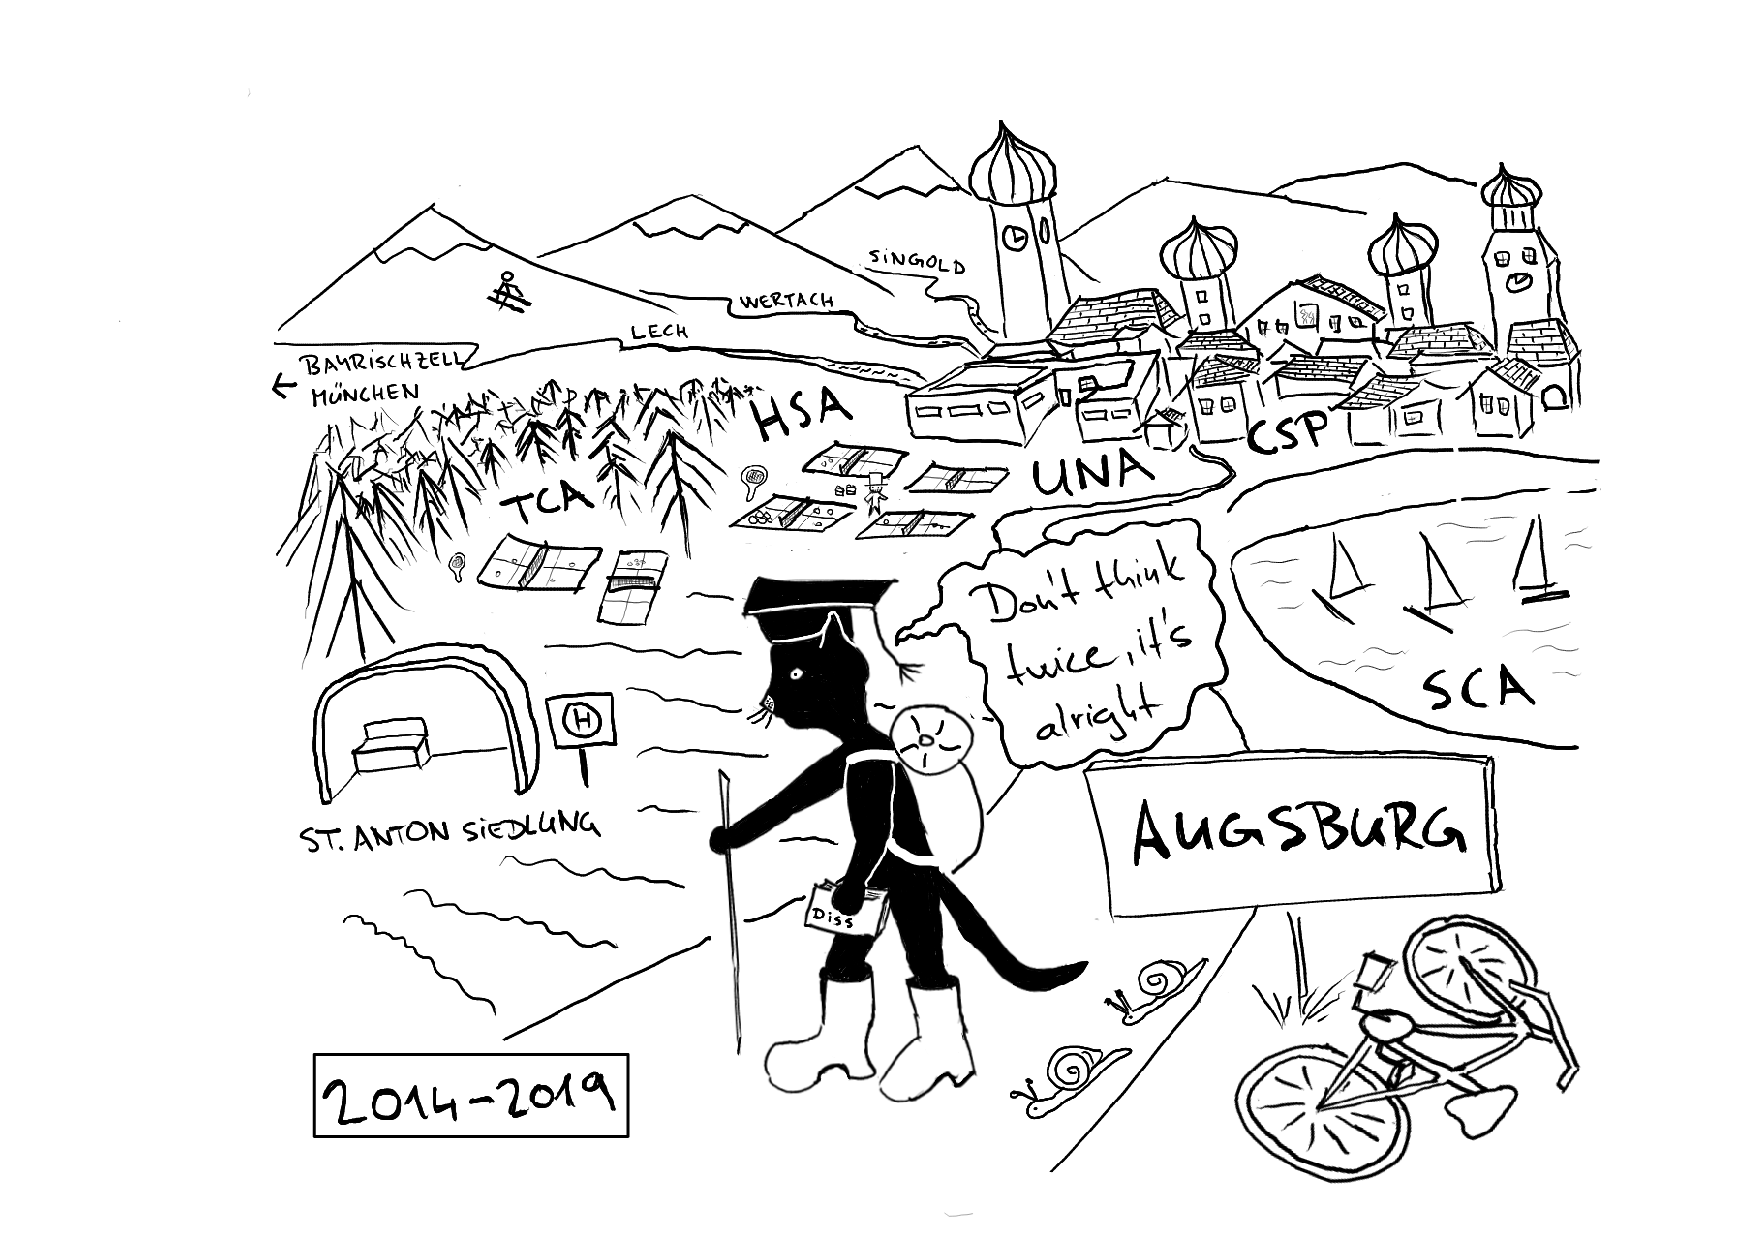
\includegraphics[trim=130 28 75 57, clip, scale=.64]{\GraphicsFolder/mikes.pdf}
%\caption[Introductory art]{Inspired by my favorite fairy tale character Kater Mikesch.}
\end{figure}
%
%I was 3 years lost (out of it one year on another project) but in the last year, did the main computation in the 4-th year and everything made sense and started fitting together in the 5-th year.
%It is mainly the question of values which changed dramatically in my case. I thought I could. B. The last year, however, was 

%Basically all work in this thesis from January 2018 to July 2019. The years before and values. I still do not know. I would, fu*k the internet! I did not feel particularly good with. I was also definitely not work oriented. Kai told that the thesis is the last opportunity to write what I want, so let be it. The problem of Ph.D. is that one gets the feedback first after very long time.

%Report of my Ph.D. which took 5 years. The reason for this is to keep memory, share the experience, and because I think it over all the time and have the tendency to tell it to someone. I hope that by writing it down it stops haunting me. If you think this does not belong to a scientific work and you are not interested in it, you can just skip it. I don't want to do the same mistakes again. There is no experiment in mathematics so I am the machine who produced it so this is basically a description how the results were obtained. Not knowing about personal situation, my skills.
%\begin{itemize}
%\item 
%\item I basically tried to work without studying that much. The task I got after the first year was to compute the example of $\Sph{n}$ by an attempt to compute the propagator for $\Sph{3}$ in spherical ideas. I basically got stuck because the computation were unmanageable.
%\item The reason I did not get depressed earlier was that there were many thing to do Witten's papers, homotopy algebra, $\BV$-formalism, Chern-Simons theory, teaching in German, giving talks in seminars, conferences traveling, learning much. And because nowadays, if you are unhappy you just live on the internet. I also did my hobbies a lot (in comparison when I basically dropped my hobbies). Whenever I felt like I did not have anything concrete to work on which I also kept telling my peers. Cryptocurrency and stock trading episode which took me a lot of my free time.
%\item When my supervisor told me that I should write a thesis the next year. I started thinking of this for the first time. I got depressed for the first time which led to some open discussion with my supervisor.  He proposed that I can prove that my propagator extends smoothly to the blow-up. This turned out to be manageable task which I accomplished during the summer. The next thing was to develop signs. I basically developed signs again not a part of the thesis. 
%\item On Christmas 2018-2019, when I started thinking about how to plug the integrals in the $\IBLInfty$-formalism I realized that this is not going to go anywhere. Seeing that the work so for was not going anywhere and comparison to peers plus personal issues I proposed that I would just quit. (+1 year in bachelor to write second bachelor thesis and +1 in masters from personal reasons.)
%
%I decided to close this as soon as possible 
%I started studying all the theory, discovering that there is a lot of other things to do which were doable --- like cyclic homology, etc, I also learned string topology finally. In October 2018 I was happy to close the part and write the paper, which is basically to separate the experience with computing the integrals.
%\item $95\%$ of what you are reading including learning of the theories was created since February 2018 until September 2019. Personally, it was a crazy ride.
%\end{itemize}
%
%for Answering my questions.
%\clearpage
\end{document}
